\documentclass[spanish,12pt,letterpapper]{article}
\usepackage{babel}
\usepackage[utf8]{inputenc}
\usepackage{graphicx}
\usepackage{hyperref}
\begin{document}
	\begin{titlepage}
		\begin{center}
			
\includegraphics[width=0.6\textwidth]{../logoUnADM}~\\[1cm] 
			\textsc{Universidad Abierta y a Distancia de México}\\[0.8cm]
			\textsc{Desarrollo de Software}\\[1.8cm]
			
			\textbf{ \Large Actividad 3. Artefactos UML}\\[3cm]
			
			Diego Antonio Plascencia Lara\\ ES1421004131 \\[0.4cm]
			Facilitador(a): Julia Alicia Reyes Rios\\
			Materia: Modelado de Negocios\\
			Grupo: DS-DMDN-1601-B1-007 \\
			Unidad: I \\
			
			\vfill México D.F\\{\today}
			
		\end{center}
	\end{titlepage}
	
	\section{Artefactos UML (Activity Diagrams)\\}
	\paragraph{Nodo Inicial.} Un circulo relleno, significa el inicio del diagrama, no es totalmente necesario, sin embargo hace mas fácil la lectura del diagrama.
	\paragraph{Nodo Final.} Un circulo relleno con un borde alrededor es significado del final del diagrama, y un diagrama puede tener cero o mas nodos finales.
	\paragraph{Actividad.} Los rectángulos redondeados representan actividades que ocurren, una actividad puede ser física, electrónica, etc.
	\paragraph{Flujo.} Las flechas en el diagrama, estas indican la dirección y el flujo.
	\paragraph{Bifurcación.} Una barra negra, donde entra un flujo y salen varios, significa el comienzo de actividades en paralelo.
	\paragraph{Reunión.} Una barra negra, con varios flujos entrando y uno solo saliendo, denotan el termino de las actividades en paralelo y todas ellas deben haber terminado antes de continuar.
	\paragraph{Condición.} Un diamante, con una entrada y dos salidas, nos indica que debemos continuar si se cumple una condición o regresar.
	\paragraph{Decisión.} Un diamante con una entrada y muchas salidas, indica que debemos seguir un camino, dependiendo de las condiciones o situaciones.
	\paragraph{Unión.} Un diamante con muchas entradas y una sola salida, indica que todas las actividades de los hilos que entran deben terminarse hasta este punto para poder continuar.
	\paragraph{División} Lineas en el diagrama indican la división de quien o que realiza la actividad.
	\paragraph{Sub Actividad.} Un tridente en la esquina de una actividad, indica que esta actividad tiene otro diagrama que la detalla mas.
	\paragraph{Flujo final.} Un circulo con una cruz en el, indica que si se llega a este punto, el proceso debe detenerse.
	\paragraph{Nota.} Un dibujo de una nota, con lineas puntiagudas que indican a que pertenece la nota.
	
	\section{Identificar los artefactos usados}
	En mi actividad anterior, use unicamente los artefactos mas sencillos, use 4 de actividad (rectángulos redondeados), 1 de condición y los nodos inicial y final.\\
	
	\begin{center}
	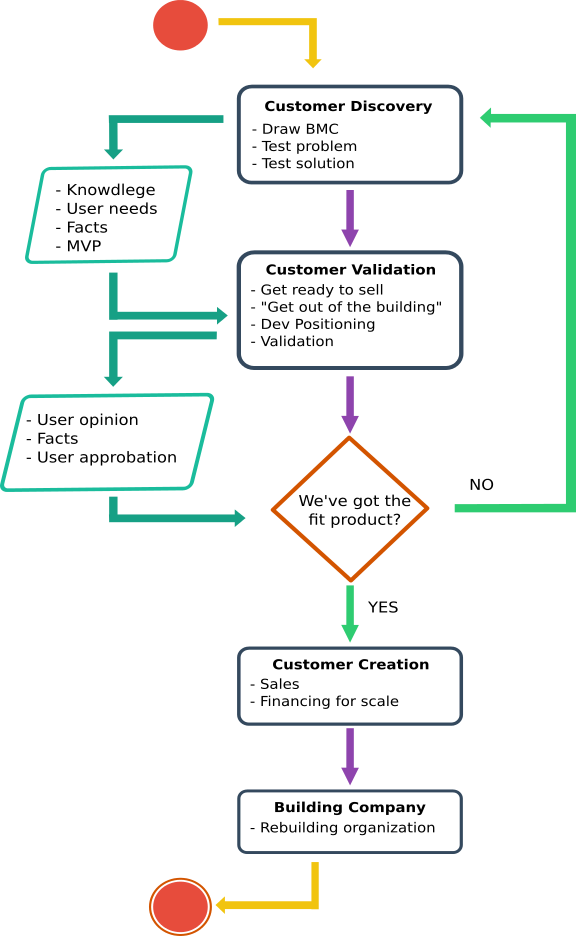
\includegraphics[width=0.4\textwidth]{./diagram}~\\[0.5cm]
	\end{center}
	
	\section{Mapa mental.}
	Puede encontrar mi mapa publico en la siguiente dirección:\\
	\url{https://atlas.mindmup.com/2016/02/8d1ac820b5b90133ea4d5f3ab3e432d0/artefactos_uml_activity_diagram/index.html}
	
	
	
	\pagebreak
	\begin{thebibliography}{9}
	\bibitem{agilemodeling} Amber, Scott W. 
		\emph{UML 2 Activity Diagrams: An Agile Introduction}. Agile Modeling {[} Fecha de consulta: \today {]}. Disponible en: \textless http://agilemodeling.com/artifacts/activityDiagram.htm \textgreater	
	
		\bibitem{maturanaModelamiento} Maturana Ortiz, Jorge. 
		\emph{Modelamiento de Software y Negocios}. {[} Fecha de consulta: \today {]}. Disponible en: \textless http://www.info.univ-angers.fr/pub/maturana/files/Modelamiento\_de\_Software\_y\_Negocios.pdf \textgreater
		
		\bibitem{wikipediaUML} Wikipedia, the free encyclopedia. 
		\emph{Unified Modeling Language}. {[} Fecha de consulta: \today {]}. Disponible en: \textless https://en.wikipedia.org/wiki/Unified\_Modeling\_Language \textgreater
		
		\bibitem{panAdm} León León, Oyuky María \& Asato España, Julio Armando. 
		\emph{La Importancia del Modelado de Procesos de
			Negocio como Herramienta para la Mejora e
			Innovación}. Panorama administrativo {[}en linea{]}, México. 2009, vol.4 num. 7  {[} Fecha de consulta: \today {]}. Disponible en: \textless http://132.248.9.34/hevila/Panoramaadministrativo/2009/no7/4.pdf \textgreater
	\end{thebibliography}
\end{document}